\chapter{Radio Galaxies}

\section{Active Galactic Nuclei}
Galaxy is gravitationally-bound system of stars, gas, dust, and dark matter. A galaxy is said to be active when its radiation shows evidence of energy source other than the known processes associated with stars, i.e. spectral distribution of the radiation from such galaxies cannot be described by a superposition of
the spectra of their stellar population. Sign of the activity of the galaxy usually associated with a very compact region at the center of the galaxy. Therefore, an active galaxy is said to host an active galactic nucleus.

Moreover, Active Galactic Nuclei (AGN) are compact regions at the center of galaxies  with a supermassive black hole (SMBH) as central engine causing an emission much stronger than the stellar emission of the entire galaxy. The strong gravitational potential of the SMBH pulls the surrounding materials inwards, forming an accretion disc of hot plasma often with additional structure of relativistic jets \citep{netzer2013}.

The continuum radiation from AGN stretches over the entire range of the electromagnetic spectrum, from the radio to the $\gamma$-ray region. The continuum spectrum has an overall complex shape, i.e., very different from the simple blackbody emission or a stellar source. However, it can often be approximated by a simple power law form over fairly wide wavelength intervals, that is,
\begin{equation}
\label{eq:fluxdensity}
S(\nu) \varpropto \nu^{-\alpha},
\end{equation}
where $S(\nu)$ is the flux density at a specific frequency $\nu$ and $\alpha$ is the spectral index. The radiation is mainly emitted through (non-thermal) processes such as synchrotron emission, bremsstrahlung and inverse Compton scattering, and modified by scattering, absorption and reemission \citep{kembhavi1999}. AGN often show variability that depends on wavelength with various time scales, ranging from minutes to years.  As mentioned earlier, active galaxies, especially radio-loud galaxies, can be detected at large distances, making them valuable tools for observational cosmology. \autoref{fig:qso_z} shows the quasar distribution from Sloan Digital Sky Survey (SDSS) Quasar Catalog (12th Data Release) appear in \cite{paris2017}. Recent observations show that the first galaxies and stars are already formed in $z = 6$ (correspond to the age of universe $\sim 1$ Gyr, using standard model cosmology).

\begin{figure}[!ht]
\centering
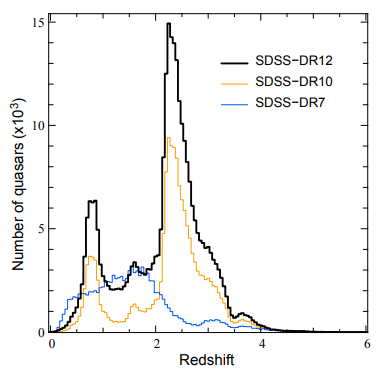
\includegraphics[scale=0.5]{fig/redshift.png}
\caption[Redshift distribution of quasars from the SDSS]{Redshift distribution of the SDSS-DR12 (thick black histogram), SDSS-DR10 (orange histogram) and SDSS-DR7 (blue-histogram) quasars over the redshift range 0-6. The two peaks at $z \sim 0.8$ and $z \sim 1.6$ seen in the SDSS-DR10 and SDSS-DR12 redshift distributions are due to known degeneracies in the SDSS color space \citep{paris2017}.}
\label{fig:qso_z}
\end{figure}


\subsection{Classification and Unification}

Many classes of AGN, names, and terminology appear in literature mainly due to historical observational reasons. To understand the physics and evolution of active galactic nuclei, we usually start with the classification and unification of these objects. 

On the first step, one can differentiate AGNs into radio-loud and radio-quiet sources. To separate radio-loud from radio-quiet AGNs, we can define ``radio-loudness'' parameter, $R$, as fraction between flux density observed at radio 
($S_{\text{radio}}$, at 5 GHz) and at optical wavelength ($S_{\text{optic}}$, at 4400 \AA),
\begin{equation}
R_{ro}  = \frac{S_{\text{radio}}}{S_{\text{optic}}}.
\label{eq:loudness}
\end{equation} 
The dividing line between radio-loud and radio-quiet AGNs is usually set at $R_{ro} = 10$ \citep{kellermann1989}. The next step we can try to distinguish AGN by their emission spectrum/lines, which leads to the so called AGN-\textit{zoo}. Generally, radio-quiet sources can be differentiated into Seyfert galaxies and radio-quiet quasars, while radio-loud sources can be divided into radio-loud quasars, blazars and radio galaxies. 

\begin{figure}[!ht]
\centering
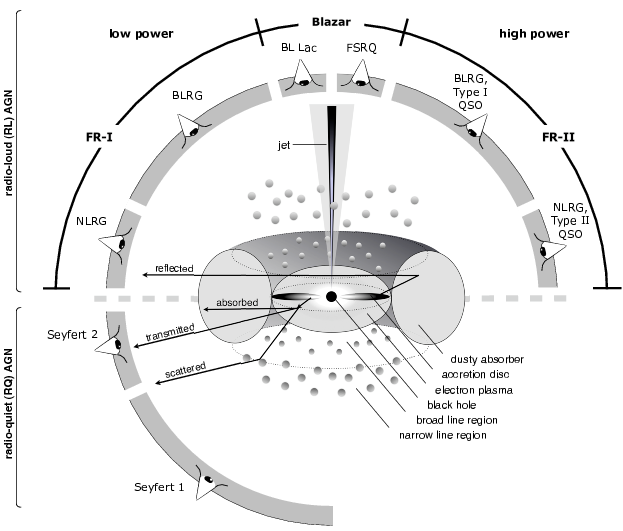
\includegraphics[width=0.85\textwidth]{fig/AGN_unification_Beckmann_Shrader_2012.png}
\caption[Schematic representation of our understanding of the AGN phenomenon in the unified scheme]{Schematic representation of our understanding of the AGN phenomenon in the unified scheme. Graphic by Marie-Luise Menzel, adopted from \cite{beckmann2012}.}
\label{fig:agn_unif1}
\end{figure}

The idea of AGN unification was proposed by \cite{antonucci1993} who suggests that the diversity of AGN can be explained with two parameters: the torus inclination with respect to the line of sight (LOS) and the source luminosity (see \autoref{fig:agn_unif1}). This scheme is perhaps the simplest possible way to characterize the known fact that the nuclear continuum and emission line radiation of AGN can suffer from wavelength-dependent scattering, absorption, and reflection on the way out. This model can account for the different observed properties of emission lines in IR, optical, and UV; the luminosity and variability of the optical-UV continuum; the different amount of obscurity of the central X-ray source. However, it is not as successful in the limits of the very low and very high luminosity, where the presence of such obscurer is questionable \citep{netzer2013}.  

\cite{heckman2014} proposed the next stage of unification model. They classified AGNs into two major groups: radiative-mode AGN and jet-mode AGN. Most of the energy output in radiative-mode AGN is in the form of electromagnetic radiation and is a direct result of matter accretion through a central optically thick accretion disk. On the other hand, jet-mode AGN emit primary energy output in form of bulk kinetic energy transported in two-sided jets. Their typical Eddington ratio is much smaller and jets are most likely powered via radiatively inefficient accretion flows (RIAFs).

In the unified model, radio galaxies and radio-loud quasars both belong to the same parent population \citep{urry1995}. However, there is also an alternative paradigm that recently has been gaining attention in which obscured AGN (e.g. radio galaxies) can evolve into quasar-type AGN as their merger-triggered, dust-obscured AGN become more powerful and clear out the environment \citep[e.g.,][]{hopkins2006}. In this dynamic model, radio galaxies and radio-loud quasars trace different phases in the evolution of powerful AGN and are potentially associated with different environments.

\subsection{Emission Processes}

Radiation sources can be divided into thermal and non-thermal. Thermal emission is produced by a source whose emitting materials are in local thermodynamic equilibrium (LTE). Otherwise, nonthermal emission is produced. Active galaxy or radio galaxy, emit radiation throughout the entire electromagnetic spectrum. The origin of the high-energy emission is still unclear, but in low-energy case or low frequency (e.g., in radio wavelengths), the radiation source (i.e., continuum) is dominated by synchrotron, and dust emission. Only small fraction of energy comes from free-free emission. 

\subsubsection{Synchrotron Emission}

Any accelerated charged particle will emit electromagnetic radiation with power specified by Larmor's formula (nonrelativistic). In astrophysical situations, electromagnetic forces produce the strongest accelerations of charged particles. Acceleration by an electric field accounts for free-free radiation. Acceleration by a magnetic field produces \textit{magnetobremsstrahlung}, the German word for ``magnetic braking radiation''. Electron (and positron if present) is the lightest particle compared to the massive proton/ion. Hence, electrons account for virtually all of the radiation observed.

Consider an electron with energy $E$ that is moving in a uniform magnetic field $B$ of energy density $u_B = B^2/8\pi$. The energy loss rate, $-dE/dt$, which is also the power emitted by the electron, $P$, is given by
\begin{equation}
P = 2 \sigma_T c \gamma^2 \beta^2 u_B \sin^2{\alpha},
\end{equation}
where $\sigma_T$ is the Thomson cross section, $c$ is the speed of light, $\gamma$ is the Lorentz factor, and $\beta = v/c$, where $v$ is the speed of the electron. The angular term $\sin^2{\alpha}$ reflects the direction of motion, where $\alpha$ is the pitch angle between the direction of motion and the magnetic field. Averaging over isotropic pitch angles gives
\begin{equation}
\overline{P} = \frac{4}{3} \sigma_T c \gamma^2 \beta^2 u_B.
\end{equation}

The radiation emitted by a single electron is beamed in the direction of motion. The spectral energy distribution (SED) of this radiation is obtained by considering gyro frequency of the electrons around the field lines ($\omega_B = e B / \gamma m_e c$) and the mean interval between pulses ($2 \pi / \omega_B$). The calculation of pulse width is obtained by considering the relativistic time transformation between the electron frame and the observer frame. This involves and additional factor of $\gamma^2$. Thus the pulse width is proportional to $\gamma^{-3}$ or, expressed in Larmor angular frequency, $\omega_L = e B/ m_e c$, to $\gamma^{-2}$. Fourier transforming these expressions gives the mean emitted spectrum of a single electron, $\overline{P}_{\nu}(\gamma)$, which peaks at a frequency near $\gamma^2 \omega_L$.

Assume now a collection of electrons with an energy distribution ($n(\gamma)d\gamma$) that gives the number of electrons per unit volume with $\gamma$ in the range of $\gamma$ to $\gamma + d\gamma$. The emission coefficient due to electrons can be obtained by summing $\overline{P}_{\nu}(\gamma)$ over all energies
\begin{equation}
j_{\nu} = \frac{1}{4\pi}\int_{1}^{\infty} \overline{P}_{\nu}(\gamma) n(\gamma) d\gamma.
\end{equation}
There is no general analytical solution to this expression since $n(\gamma)$ can take various differents forms. However, there are several cases of interest where $n(\gamma)$ can be represented as a power law in energy $n(\gamma)d\gamma = n_0 \gamma^{-p} d\gamma$. The additional assumption that all the radiation peaks around a characteristic frequency $\gamma^2 \nu_L$, where $\nu_L$ is the Larmor frequency, gives the following solution for $j_\nu$
\begin{equation}
4 \pi j_\nu = \frac{2}{3} \sigma_{T} n_0 u_B \nu_{L}^{-1} \left( \frac{\nu}{\nu_L} \right)^{-\frac{p-1}{2}}
\end{equation}
Consider $p = 2.5$, which is expected in various important cases, for example, particles accelerated by relativistic shocks. This  gives $j_\nu \varpropto \nu^{-0.75}$. To obtain the monochromatic luminosity ($L_\nu$) of an optically thin medium emiting synchotron radiation, we must integrate over the volume of the source,
\begin{equation}
L_\nu = \int_{V} j_\nu dV \varpropto \nu^{-0.75}
\end{equation}
This is similar to the observed continuum slope of many AGNs at radio, optical, UV and X-ray energies (see \autoref{eq:fluxdensity}).

The source of fast electrons can be opaque to its own radiation. This results in a significant modification of the emergent spectrum, especially at low frequencies, where the opacity is the largest. This case is usually called synchrotron self-absorption mechanism and the resulted specific intensity will be proportional to $\nu^{5/2}$, which describes the synchrotron SED at low energies. Concerning this work, using ALMA, this synchrotron radiation can 
be measured in Band 3.

\subsubsection{Dust Emission}

After synchotron, the second most important source of radiation/continuum in low frequencies from an active galaxy is dust emission. All small solid particle in space is called dust grains by astronomers. Interstellar dust was first recognized from their extinction (i.e., scattering and absorption) properties in far-infrared (FIR), optical, and UV wavelengths. Interstellar dust grains are much smaller than common terrestrial dust particles visible to the naked eye, and they are much smaller than the wavelengths $\lambda > 300$ $\mu$m (frequencies $\nu < 1$ THz) accessible to ground-based radio astronomy such as ALMA.

Dust scattering occurs due to oscillating electric field of incident radiation that forces electrons within dust grain to oscillate and, thus, reradiate at the same frequency in all directions.  In the limit $\lambda \gg a$, where $a$ is the size of the grains, these radiators are very inefficient, so their scattering cross section is proportional to $\lambda^{-4}$ (Rayleigh's law). Some of the incident photons are not scattered, but absorbed by the dust grains, which in turn will heat the dust grains. The energy by a single UV photon can significantly raise the temperature of a very small dust grain, so the smallest dust grains are not in thermodynamic equilibrium with the local interstellar radiation field. 

In fact, larger interstellar dust grains have enough heat capacity to come into equilibrium at well-defined temperatures ($20 < T_d({\rm K})<200$), such that the power absorbed is balanced by power reemitted primarily at  FIR wavelengths. At radio wavelengths, the dust absorption contributes much more than dust scattering to the total extinction. One type of galaxy called starburst galaxy, which has very high star formation rate, are very bright in the IR region due to this dust heating process.

%All galaxies are nearly transparent, thus from radio observations, we can see into the dusty starburst galaxies, and the radio luminosity is nearly proportional to the recent rate of star formation, unaffected by dust extinction.

The dusty radio sources do not have Rayleigh-Jeans radio spectra $S_\nu \varpropto \nu^{2}$; they have relatively a spectra rising as $S_\nu \varpropto \nu^{2 + \beta}$ with $1 < \beta < 2$. A striking consequence of such a steeply rising spectrum is that the flux density of a galaxy observed through the atmospheric window (at $\lambda \sim 1$ mm or $\nu \sim 300$, ALMA Band 6 and 7) is nearly independent of its redshift in the range $1 < z < 10$. The strongest submm galaxies tend to be the most luminous, and radio surveys at wavelengths near $\lambda \sim 1$ mm are effective at tracing the rate of star formation over the entire redshift range during which most stars formed \citep[e.g.,][]{blain1993}.

\section{Radio Galaxy}

As previously mentioned, being a member of radio-loud AGN, radio galaxies are types of active galaxy that have enormous radio luminosities \citep[e.g.][]{miley2008, netzer2013, heckman2014}. Because it is luminous, radio-loud active galaxies can be detected at very large distances using the appropriate radio telescopes. Therefore, the distant universe can be probed using these radio-loud active galaxies to provide different information for cosmology. 

The difference between radio galaxy and other member of radio-loud AGN is the resolvable jet structure. The observed structure in radio emission is determined by the interaction between twin jets and the external medium, modified by the effects of relativistic beaming. In optical wavelength they can be divided in two sub-classes: Broad line radio galaxies (BLRG) have emission lines resembling those from Seyfert 1 galaxies, while narrow line radio galaxies (NLRG) have spectra like the Seyfert 2 galaxies. Recently, much work has been done on the effects of these objects on the intergalactic medium, particularly in galaxy groups and clusters. It is important to note that the term radio galaxy in this dissertation will be used not only for the resolvable radio-loud AGN, but for all of them.

\subsection{Morphology}

Unlike quasar, `resolvable radio galaxies' display wide range of radio structures. The most common large scale structures are called lobe, hotspot, jet, and sometime plume (see \autoref{fig:fr}). \textit{Lobes} are roughly ellipsoid structure, usually double and fairly symmetrical on either side of nucleus. In rather low luminosity case, it is often called \textit{plumes}. Some radio galaxies show one or two narrow features known as \textit{jets}, directly coming from nucleus and going to the lobes. It is believed that lobes or plumes are powered or supplied by high-energetic particles and magnetic fields from active nucleus through this jets \citep[see, e.g., ][]{scheuer1974, blandford1974}.

\begin{figure}[!ht]
\centering
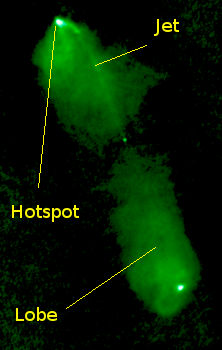
\includegraphics[width=0.49\textwidth]{fig/Radio_galaxy_3C98.png}
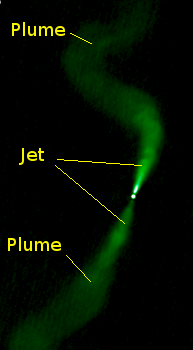
\includegraphics[width=0.425\textwidth]{fig/Radio_galaxy_3C31.png}
\caption[Example of radio image for the FR I and FR II radio galaxy]{(Left) Radio image of FR II radio galaxy, 3C98. (Right) Radio image of FR I radio galaxy, 3C31. Labelled in the image are structures usually found in radio galaxy: lobes, jets, hotspot, and plumes.}
\label{fig:fr}
\end{figure}

\cite{fanaroff1974} divided radio galaxies into two clasess based on their morphology, i.e., FR I and FR II. While FR I are radio galaxies that have brighter spot located at the center of active nuclei and gradually decrease, FR II are radio galaxies that have brighter spots located at the far edge of the jet/lobes. Furthermore, \cite{fanaroff1974} found that FR II are more luminous than FR I. In some cases, we cannot classify the class of radio galaxy, either as FR I or FR II. On the other hand, there is a hybrid case in which FR I is seen on one lobe and FR II on the other lobe. With more detailed radio observations, the morphology reflects the mechanism of energy transport in the radio source. Consequently, the environment of radio galaxies plays important roles.

It also has been argued that FR II radio galaxies, are triggered by molecular gas fed towards the center \citep{buttiglione2010}, while the FR I type are triggered through a ``dry'' accretion (Bondi accretion) in the Broad Line Region (BLR, see \citep{fromerth2001}). A key aspect is the ability to feed the accretion disk around the central Supermassive Black Hole (SMBH, see \cite{merloni2008}). It has been suggested that ``wet'' minor mergers would be a mechanism to bring molecular gas and dust towards the center of the radio galaxies and trigger the radio activity \citep[e.g.,][]{lim2000, israel1998}.

\subsection{Host Galaxies and Environments}

Observations have shown that radio-loud AGN usually reside in overdense environments \citep[see, e.g.,][]{stevens2003, venemans2007, falder2010, galametz2010b, galametz2012, mayo2012}. The host galaxies are almost exclusively large and massive elliptical galaxies. If the radio jets are not in the LOS, the central black hole in radio galaxies is usually obscured by a thick dust torus and does not outshine the host galaxy. Therefore, investigating the SED of radio galaxies enables one to study their host galaxy's stellar, dust and AGN components. Nevertheless, for a distant-unresolvable radio galaxy, it will be difficult to disentangle these components, because we don't have any information about the orientation of the radio jet.

Radio galaxies are very luminous in FIR regime indicating very high star-formation rates. Observations show that star-formation rates in radio galaxies can reach several thousands $M_{\odot}$/yr \cite[e.g.,][]{archibald2001, drouart2014}. Moreover, \cite{miley2008} found that their sub-millimeter luminosity increases with redshift, implying that star-formation rates were higher at early times. Nevertheless, it is also difficult to disentangle the source of dust heating process: by AGN or stars. It requires detailed modelling and SED fitting of each component. Observation on Rayleigh-Jeans tail of the sub-millimeter region is crucial as it may constrain the slope of the dust emission heated by stars \citep{drouart2014}. This tail is also important for deriving far-infrared photometric redshifts \citep{wylezalek2013b}.  ALMA frequency is important because it is located in this region. Catalogue of SED produced in this work will be useful to disentangle the source of dust heating process in radio galaxies, which will then be useful to correctly measure the star formation rates.


% Equally interesting is their likely effect on structure formation over cosmological time: it is thought that they may provide a feedback mechanism to slow the formation of the most massive objects.

\cleardoublepage
